% \usetikzlibrary{patterns} % Load patterns library
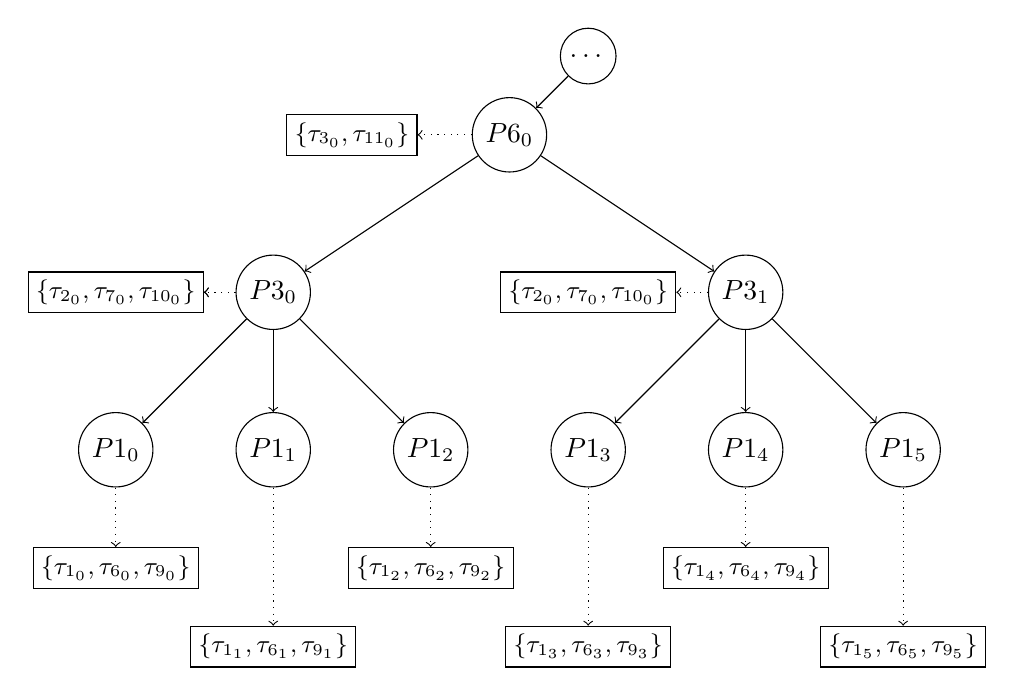
\begin{tikzpicture}
	\node[draw, circle, inner sep=1mm] (L2-00) at ( 6, 5) {\ldots};

	\node[draw, circle, inner sep=1mm] (L3-00) at ( 5 , 4) {$P6_0$};

	\node[draw, circle, inner sep=1mm] (L4-00) at ( 2 , 2) {$P3_0$};
	\node[draw, circle, inner sep=1mm] (L4-01) at ( 8 , 2) {$P3_1$};

	\node[draw, circle, inner sep=1mm] (L5-00) at ( 0 , 0) {$P1_0$};
	\node[draw, circle, inner sep=1mm] (L5-01) at ( 2 , 0) {$P1_1$};
	\node[draw, circle, inner sep=1mm] (L5-02) at ( 4 , 0) {$P1_2$};
	\node[draw, circle, inner sep=1mm] (L5-03) at ( 6 , 0) {$P1_3$};
	\node[draw, circle, inner sep=1mm] (L5-04) at ( 8 , 0) {$P1_4$};
	\node[draw, circle, inner sep=1mm] (L5-05) at (10 , 0) {$P1_5$};

	\node[draw, rectangle, inner sep=1mm, align=center] (L3-T00) at ( 3 , 4) {\small $\{\tau_{3_0},\tau_{11_0}\}$};

	\node[draw, rectangle, inner sep=1mm, align=center] (L4-T00) at ( 0 , 2) {\small $\{\tau_{2_0},\tau_{7_0},\tau_{10_0}\}$};
	\node[draw, rectangle, inner sep=1mm, align=center] (L4-T01) at ( 6 , 2) {\small $\{\tau_{2_0},\tau_{7_0},\tau_{10_0}\}$};

	\node[draw, rectangle, inner sep=1mm, align=center] (L5-T00) at ( 0 , -1.5) {\small $\{\tau_{1_0},\tau_{6_0},\tau_{9_0}\}$};
	\node[draw, rectangle, inner sep=1mm, align=center] (L5-T01) at ( 2 , -2.5) {\small $\{\tau_{1_1},\tau_{6_1},\tau_{9_1}\}$};
	\node[draw, rectangle, inner sep=1mm, align=center] (L5-T02) at ( 4 , -1.5) {\small $\{\tau_{1_2},\tau_{6_2},\tau_{9_2}\}$};
	\node[draw, rectangle, inner sep=1mm, align=center] (L5-T03) at ( 6 , -2.5) {\small $\{\tau_{1_3},\tau_{6_3},\tau_{9_3}\}$};
	\node[draw, rectangle, inner sep=1mm, align=center] (L5-T04) at ( 8 , -1.5) {\small $\{\tau_{1_4},\tau_{6_4},\tau_{9_4}\}$};
	\node[draw, rectangle, inner sep=1mm, align=center] (L5-T05) at (10 , -2.5) {\small $\{\tau_{1_5},\tau_{6_5},\tau_{9_5}\}$};

	\draw[->] (L2-00) to (L3-00);

	\draw[->] (L3-00) to (L4-00);
	\draw[->] (L3-00) to (L4-01);

	\draw[->] (L4-00) to (L5-00);
	\draw[->] (L4-00) to (L5-01);
	\draw[->] (L4-00) to (L5-02);
	\draw[->] (L4-01) to (L5-03);
	\draw[->] (L4-01) to (L5-04);
	\draw[->] (L4-01) to (L5-05);

	\draw[->,dotted] (L3-00) to (L3-T00);
	\draw[->,dotted] (L4-00) to (L4-T00);
	\draw[->,dotted] (L4-00) to (L4-T00);
	\draw[->,dotted] (L4-01) to (L4-T01);
	\draw[->,dotted] (L5-00) to (L5-T00);
	\draw[->,dotted] (L5-01) to (L5-T01);
	\draw[->,dotted] (L5-02) to (L5-T02);
	\draw[->,dotted] (L5-03) to (L5-T03);
	\draw[->,dotted] (L5-04) to (L5-T04);
	\draw[->,dotted] (L5-05) to (L5-T05);

\end{tikzpicture}